%%%%%%%%%%%%%%%%%%%%%%%%%%%%%%%%%%%%%%%%%%%%%%%%%%%%%%%%%%%
\frame{
\frametitle{My slide title}

    % some bullet points
    \begin{textblock*}{60mm}(10mm,25mm)
        \begin{itemize}
            \item[$\rightarrow$] Point 1
            \item[$\rightarrow$] Point 2 which is much longer so one can see the box width
            \only<2>{\item[$\rightarrow$] Point 3}
        \end{itemize}
    \end{textblock*}

    % figure
    \begin{textblock*}{80mm}(75mm,10mm)
        \centering
        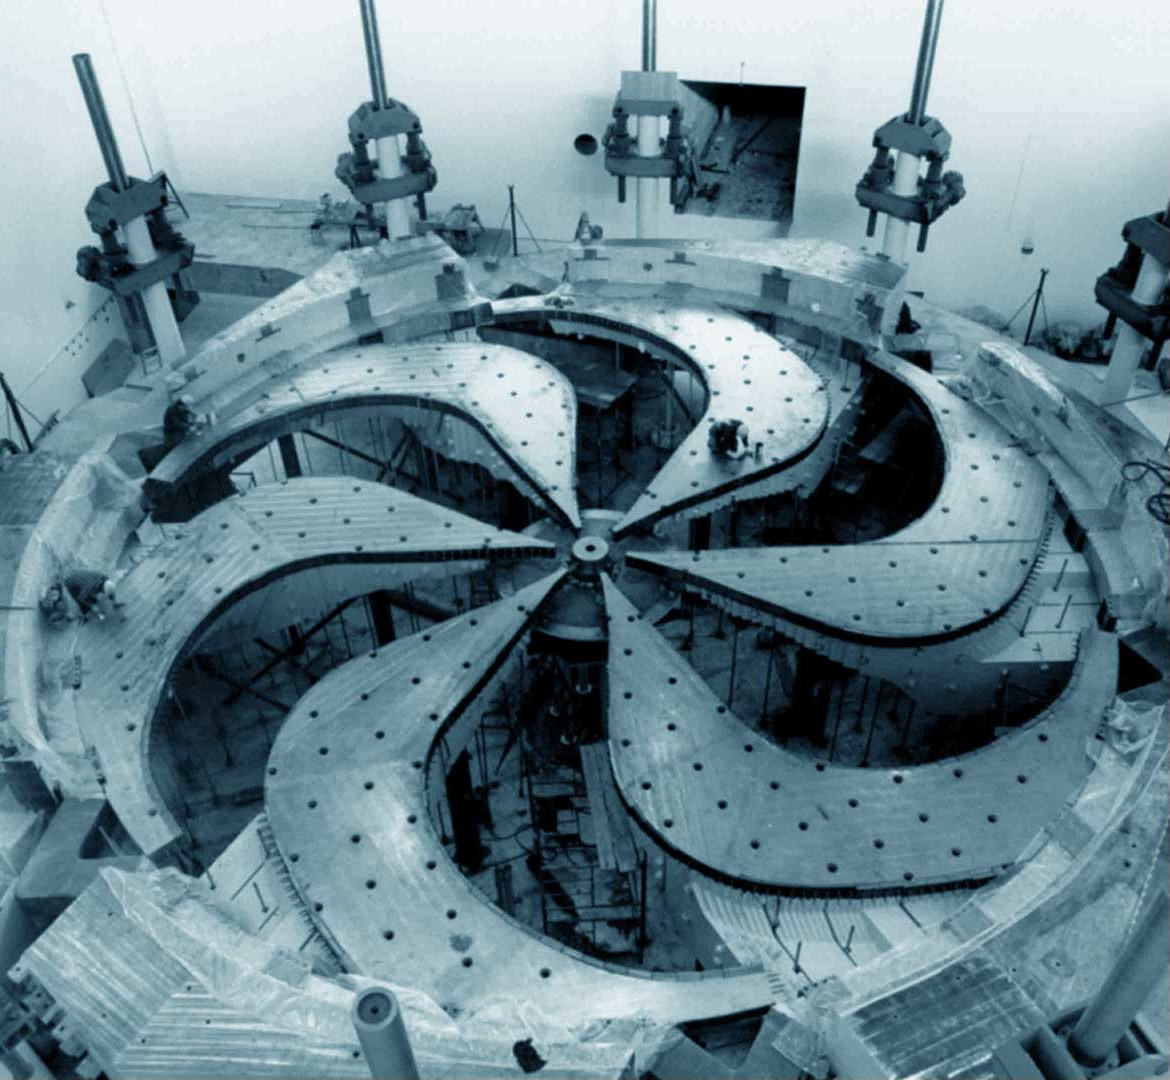
\includegraphics[keepaspectratio=true,width=\textwidth,trim= 0cm 0cm 0cm 0cm, clip=true]{cyc1.jpg}
    \end{textblock*}
}
